\documentclass{article}
\usepackage{tikz}
\usepackage{multicol}
\usepackage[margin=1in]{geometry}

\newcommand{\blanktable}{\begin{tabular}{l|c|c|}
 Test & \multicolumn{2}{c}{Person}\\
 Result & Criminal & Innocent\\\hline
 Pos. & & \\\hline
 Neg. & & \\\hline\hline
 Total & 8 & 12\\
 \end{tabular}}

\begin{document}

\pagestyle{empty}
\centerline{\Large \sffamily Math 125: Epidemiology}

\bigskip

\centerline{\Large \sffamily \bfseries In-Class Activity: Testing a Lie Detector}

\vspace*{.25in}

\noindent In 2002, the Minneapolis {\em Star Tribune} reported front-page news: a new technology with the potential to screen terrorists at airports:

\bigskip

\centerline{\Large \bf Seeing through the mask of deceit}

\begin{multicols}{2}
\noindent Jill Burcum

\noindent {\em 3 January 2002, p. A1}

\bigskip

The old childhood taunt --- ``Liar, liar pants on fire" --- may need a slight revision.

Researchers at the Mayo Clinic and Honeywell Laboratories say their new lie-detection device spots deceitful people by measuring the heat they emit from their faces.

\centerline{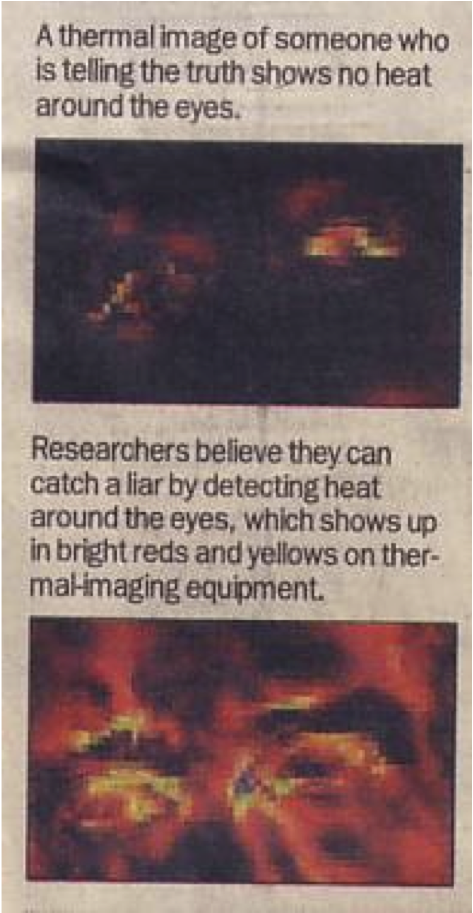
\includegraphics[width=1.5in]{thermal-image.png}}

The discovery could lead to a new, less-intrusive way to screen for terrorists at airports, they said.

When people lie, the area around the eyes gets warm while the cheeks cool, said Mayo researcher Dr. James Levine. The result, he said, is a mask-shaped pattern of heat on the liar's face.

The naked eye can't see this. But Levine and Honeywell researchers found that thermal-imaging technology can.

In a study paid for by the Defense Department and conducted at its Polygraph Institute in South Carolina, Mayo and Honeywell researchers used thermal imaging to assess whether test subjects were truthful about a mock crime.

Eight of 20 people tested were told to stab a mannequin and steal \$20 from it.  The remaining 12 did not commit this crime.

Researchers then scanned the volunteers faces when they answered questions about the mannequin and the money.

The thermal-imaging syatem correctly determined whether the volunteers were lying 83 percent of the time.

Polygraphs performed on the same people by the department's experts correctly categorized the liars and truthful people 70 percent of the time.


\end{multicols}

\noindent\hrulefill


\bigskip

The quoted accuracy of the thermal-imaging system is 83\%, suggesting that 16.6 of the 20 volunteers were correctly classified.  Of course, the number needs to be an integer, so let's assume that the thermal-imaging test correctly classified 17 of the 20, whereas the polygraph test correctly classified 14 of the 20 volunteers.

Fill in the tables in different ways consistent with the 17/20 accuracy.

\bigskip

\noindent \hbox{\blanktable \hspace{1cm} \blanktable \hspace{1cm} \blanktable}

\begin{itemize}
\item For each of your tables, calculate the sensitivity and specificity of the test.

\item Assuming that the prevalance of terrorism in airports is 1 per 1,000,000, calculate the false positive and false negative rates for each of your tables.
\end{itemize}
\end{document}